\documentclass{beamer}

\usepackage{graphicx}

\setbeamertemplate{navigation symbols}{}

\begin{document}
\begin{frame}[fragile]
\verb|[H]C1=C(N(C(=C1[H])C(=S)N=P(N(C([H])([H]|
\verb|)[H])C([H])([H])[H])(N(C([H])([H])[H])C(|
\verb|[H])([H])[H])N(C([H])([H])[H])C([H])([H]|
\verb|)[H])C([H])([H])[H])[H]|

\begin{figure}
    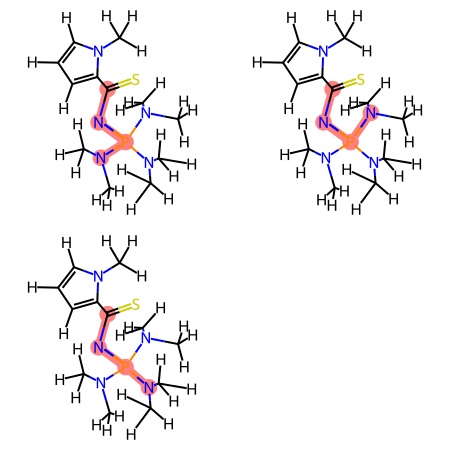
\includegraphics[width=0.7\textwidth,height=0.7\textheight,keepaspectratio]{mol01.png}
\end{figure}
\end{frame}
\begin{frame}[fragile]
\verb|[H]C1=C(N(C(=C1[H])C(=S)N=P(N(C([H])([H]|
\verb|)[H])C([H])([H])[H])(N(C([H])([H])[H])C(|
\verb|[H])([H])[H])N(C([H])([H])[H])C([H])([H]|
\verb|)[H])C([H])([H])[H])[H]|

\begin{figure}
    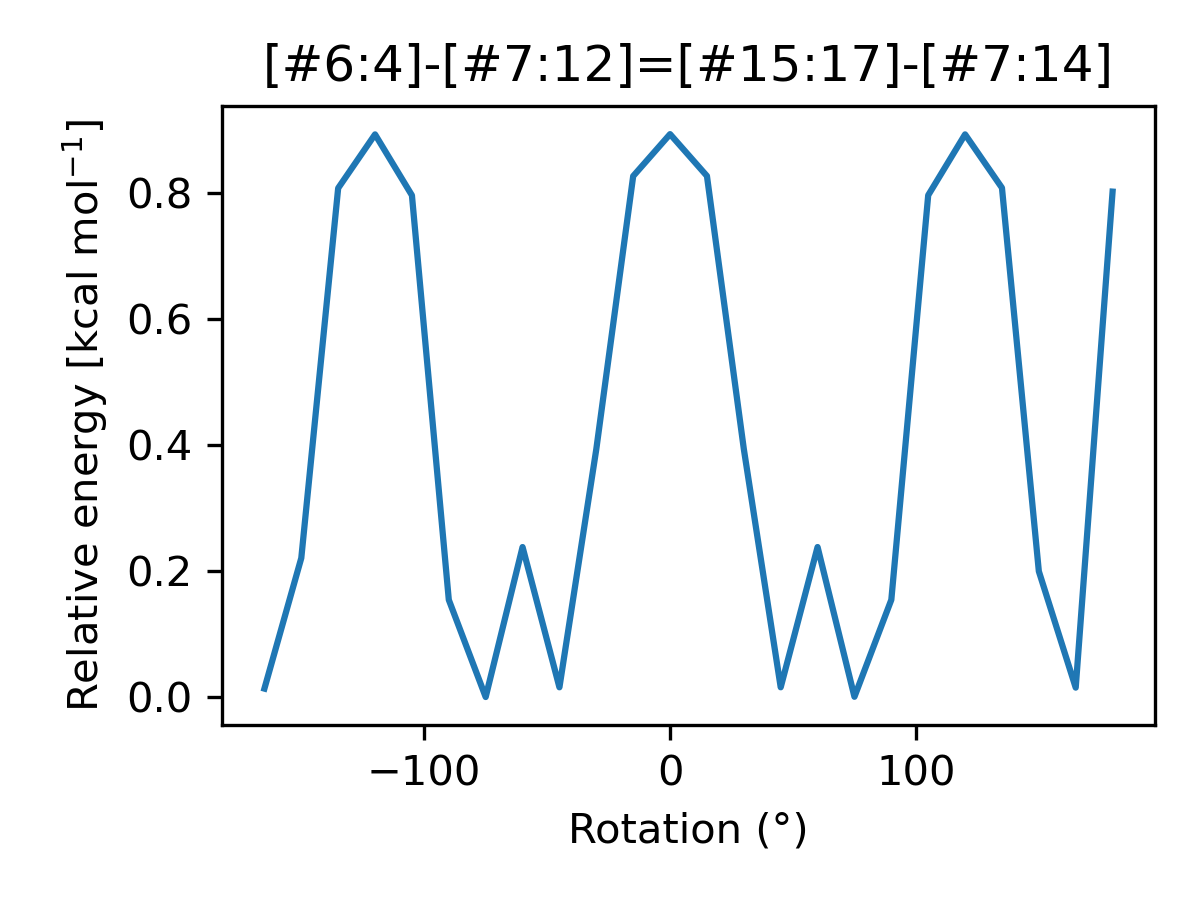
\includegraphics[width=0.7\textwidth,height=0.7\textheight,keepaspectratio]{plot01.png}
\end{figure}
\end{frame}
\end{document}